
\documentclass[10pt]{article}
\usepackage[T1]{fontenc}
\usepackage{amssymb}
\usepackage{amsmath}
\usepackage{graphicx}
% \begin{figure}[h]
% \centering
% \includegraphics[width=6.5in]{folder/photo.png}
% \caption{}
% \label{}
% \end{figure}



\usepackage{tikz}
\usetikzlibrary{arrows}
\usepackage{subfigure}
\usepackage{stackrel}
\usepackage{blindtext}

\usepackage[url=false]{biblatex}
\addbibresource{library.bib}

\oddsidemargin=0.15in
\evensidemargin=0.15in
\topmargin=-.5in
\textheight=9in
\textwidth=6.25in

\usepackage[colorlinks=true,breaklinks,pdfpagemode=none,linkcolor=blue,citecolor=blue]{hyperref}

\usepackage{enumerate}
% \vspace{-6pt}
% \begin{itemize}
%     \setlength{\itemsep}{0pt}%
%     \setlength{\parskip}{0pt}%
%     \item Item 1
%     \item Item 2
%         \begin{itemize}
%             \setlength{\itemsep}{0pt}%
%             \setlength{\parskip}{0pt}%
%             \item Sublist Item 1
%             \item Sublist Item 2
%         \end{itemize}
%         \item Item 3
% \end{itemize}
% \vspace{-6pt}


\usepackage{enumitem}
\setlist{itemsep=0mm}



%\usepackage[usenames,dvipsnames]{pstricks}
%\usepackage{epsfig}
\usepackage{amsmath,amsfonts,amssymb,bm}
%\usepackage{pst-grad} % For gradients
%\usepackage{pst-plot} % For axes



\begin{document}

   \noindent
   \begin{center}

   \hrulefill
   
   \vspace{5pt}
   
   \makebox[\textwidth]{ {\bf Energy Systems Analysis} \hfill  A.D. Smith 2019}
   \vspace{0pt}
   
   {\Large \hfill  Lecture 12. BEM: Building Systems, Part I\\ \hfill {\large Envelope, Zones, Interior}}
   \vspace{5pt}
   
  
   \hrulefill
   \end{center}

{\center{ \small{      ``Commercial buildings are complicated thermodynamic objects.''
\\%[3pt]
\rightline{{\rm --- Samuelson, Ghorayshi, and Reinhart \cite{Samuelson2016-ml}}}}}}



\section{Envelope and Construction}

The building envelope, or ``skin'' of the building, protects the building and its occupants from the elements and from a control-volume, single-building perspective, it defines your system boundary for the building. 

The building's construction, including the envelope as well as interior walls and structures, can be specified to EnergyPlus as \cite{EPcourseteaching}:

\vspace{-6pt}
\begin{itemize}
    \setlength{\itemsep}{0pt}%
    \setlength{\parskip}{0pt}%
    \item Surfaces grouped into zones
    \item Individual structures like:
        \begin{itemize}
            \setlength{\itemsep}{0pt}%
            \setlength{\parskip}{0pt}%
            \item Walls
            \item Roofs
            \item Ceilings
            \item Floors
        \end{itemize}
        \item Individual materials
        \item Groups of materials, called Constructions or Construction Sets in EnergyPlus-speak.
\end{itemize}
\vspace{-6pt}

As an EnergyPlus building simulation comes together, information from the IDF, organized according to the IDD, will be expected by EnergyPlus to fall into a hierarchy of data for processing. The hierarchy for the building's envelope is shown in Figure \ref{hierarchy}.

\begin{figure}[h]
\centering
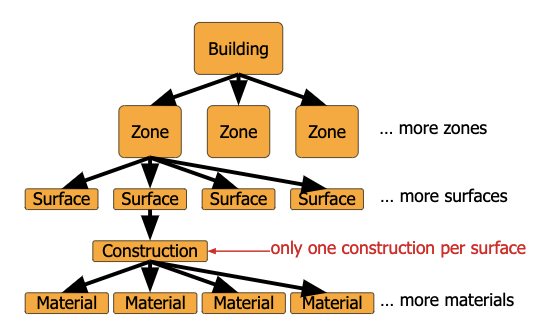
\includegraphics[width=4.5in]{extras12/envelopehierarchy.png}
\caption{Envelope Hierarchy in EnergyPlus \cite{EPcourseteaching}}
\label{hierarchy}
\end{figure}

It is a best practice to use ``as few surfaces as necessary'' \cite{EPcourseteaching}, meaning that you define a surface and reuse it for multiple walls if possible. This will require knowledge of the materials and methods used for construction, and an understanding of important phenomena at the interface of building constructions (like thermal bridging, see Lecture 8).

\section{Thermal Zoning}

Remember that the thermal zones, simply called Zones in EnergyPlus-speak, are not geometric entities but rather groups of things that will interact thermally. According to the Getting Started documentation:

\begin{quote}
    The \textbf{thermal zone} is defined as a volume of air at a uniform temperature. \cite{EPdocs9gettingstarted}
\end{quote} 

This leads to one general rule: 

\begin{quote}
Use the number of fan systems (and radiant systems) not the number of rooms to determine the
number of zones in the building. \cite{EPdocs9gettingstarted}
\end{quote}

It is best practice in any case to use ``as few zones as necessary'' \cite{EPcourseteaching}, meaning that you have just enough zones to adequately capture the phenomena that will help you make decisions based on model output, but no more zones which would add to model complexity or computational time (or likely both).\\

The rule above can be expanded toward a more systems thinking-type view of the buiding:

\begin{quote}
    The minimum number of zones in a general simulation model will
usually be equal to the number of systems serving the building. The collection of heat transfer and
heat storage surfaces defined within each zone will include all surfaces bounding or inside of the
space conditioned by the system.
\end{quote}

Making zoning decisions beyond these guidelines will require deep engineering knowledge about the interactions between building constructions, mechanical systems, occupants, and the thermal masses within the building as a whole. Furthermore, the exact same building might actually need more zones for a model that requires greater differentiation in thermal conditions within the building than it would for another, more general, model. The key is to understand how the information produced by the model will be used.

\section{Interior Environment}

\subsection{People}

People in a building are referred to as \textbf{occupants} in the world of building science. People are a type of \textbf{internal gain}, meaning that they add heat to the building's interior. For example, our skin can dissipate \textbf{latent heat} through sweating and \textbf{sensible heat} by convection or radiation.

\begin{description}
\item[Sensible heat] energy addition associated with (dry-bulb) temperature change in zone \cite{EPcourseteaching}
\item[Latent heat] energy addition associated with moisture/humidity change in zone \cite{EPcourseteaching} 
\end{description}

\subsection{Lighting}

Lighting is a type of internal gain

\subsection{Equipment}

Equipment is a type of internal gain, 

\subsection{Schedules}

Schedules describe \textit{when} things happen in the simulated building. EnergyPlus uses a nested set of schedule pieces to build unique schedules for things like lighting, equipment, and occupancy as follows \cite{EPcourseteaching}:

\vspace{-6pt}
\begin{itemize}
    \setlength{\itemsep}{0pt}%
    \setlength{\parskip}{0pt}%
    \item \textbf{DaySchedule}: 24 hour period of schedule values
    \item \textbf{WeekSchedule}: Consists of various DaySchedule definitions for an entire week
    \item \textbf{Schedule}: Consists of various WeekSchedule definitions for an entire year
\end{itemize}
\vspace{-6pt}

These can also be designated as a certain \textbf{ScheduleType}: an ``optional feature that allows for some validation and limitation of schedules.'' \cite{EPcourseteaching}


% license
\bigskip

\noindent
\texttt{\footnotesize RESTRICTED PUBLIC LICENSE --- READ BEFORE SHARING. This is a draft version made available by Amanda D. Smith under a Creative Commons Attribution-NonCommercial-ShareAlike license. 
\href{https://creativecommons.org/licenses/by-nc-sa/4.0/}{CC BY-NC-SA 4.0}}

% references
\newpage
\printbibliography

\end{document}